\documentclass[english,authoryear,12pt]{elsarticle}
%%%%%%%%%%%%%%%%%%%%%%%%%%%%%%%%%%%%%%%%%%%%%%%%%%%%%%%%%%%%%%%%%%%%%%%%%%%%%%%%%%%%%%%%%%%%%%%%%%%%%%%%%%%%%%%%%%%%%%%%%%%%%%%%%%%%%%%%%%%%%%%%%%%%%%%%%%%%%%%%%%%%%%%%%%%%%%%%%%%%%%%%%%%%%%%%%%%%%%%%%%%%%%%%%%%%%%%%%%%%%%%%%%%%%%%%%%%%%%%%%%%%%%%%%%%%
\usepackage{fullpage}
\usepackage[labelfont=bf,singlelinecheck=false,aboveskip=10pt]{caption}
%\usepackage[font={scriptsize},labelfont={scriptsize},textfont={scriptsize}]{caption}
%\DeclareCaptionFormat{myformat}{#1#2\\#3}
\usepackage{amsmath,graphicx,multicol,chngpage,setspace}
\usepackage{amssymb,amsthm,amstext,amsfonts,enumerate}
\usepackage[colorlinks=true,linkcolor=black, citecolor=blue, urlcolor=blue]{hyperref}
\usepackage[top=1in, bottom=1in, left=1.0in, right=1.0in]{geometry}
\usepackage{lscape}
\usepackage{rotating}
\usepackage{color,float,multirow,array,hyphenat}
\usepackage{booktabs}
\usepackage{subcaption}
\usepackage{natbib} % already loaded by elsarticle
\usepackage{apalike}
\usepackage{babel}
\usepackage{appendix}
\usepackage{afterpage}


\setcounter{MaxMatrixCols}{10}

% Global Document settings
%\graphicspath{{C:/Work/Papers/Murray/Projects/AIT/ait-ahmad-murray/paper/Images}}
% \linespread{1.3} % Setting it to 1.3 = 1.5 line spacing; 1.6 = double spacing
\onehalfspacing
\setlength{\parindent}{0in}
\setlength{\parskip}{1em}

% Create arg max/min operator
\DeclareMathOperator*{\argmax}{arg\,max}
\DeclareMathOperator*{\argmin}{arg\,min}
\DeclareMathOperator{\E}{\mathbb{E}}

\newcommand{\bi}{\begin{itemize}}
\newcommand{\ei}{\end{itemize}}
\newcommand{\be}{\begin{enumerate}}
\newcommand{\ee}{\end{enumerate}}
\newcommand{\bd}{\begin{description}}
\newcommand{\ed}{\end{description}}
\newcommand{\prbf}[1]{\textbf{#1}}
\newcommand{\prit}[1]{\textit{#1}}
\newcommand{\beq}{\begin{equation}}
\newcommand{\eeq}{\end{equation}}
\newcommand{\beqa}{\begin{eqnarray}}
\newcommand{\eeqa}{\end{eqnarray}}
\newcommand{\bdm}{\begin{displaymath}}
\newcommand{\edm}{\end{displaymath}}
\newcommand{\script}[1]{\begin{cal}#1\end{cal}}
\newcommand{\citee}[1]{\citename{#1} \citeyear{#1}}
\newcommand{\h}[1]{\hat{#1}}
\newcommand{\ds}{\displaystyle}


% Remove Elsevier preprint message
\makeatletter
\def\ps@pprintTitle{%
	\let\@oddhead\@empty
	\let\@evenhead\@empty
	\def\@oddfoot{}%
	\let\@evenfoot\@oddfoot}
\makeatother

\begin{document}
	\begin{frontmatter}
		\title{Implications for Determinacy with Average Inflation Targeting}
		\date{\today}
		\author[1]{Yamin Ahmad}
		\ead{ahmady@uww.edu}
		\author[2]{James Murray}
		\ead{jmurray@uwlax.edu}

		\cortext[cor1]{Corresponding author}
		\address[1]{Dept. of Economics, University of Wisconsin - Whitewater, 809 W. Starin Road, Whitewater, WI 53190, USA}
		\address[2]{Dept. of Economics, University of Wisconsin - La Crosse, 1725 State St., La Crosse, WI 54601, USA}

	\date{\today}

	\begin{abstract}
		%\renewcommand{\baselinestretch}{1.5}
		We use a three-equation New Keynesian model to explore the implications of backward- and forward-looking windows when constructing a measure for an average inflation target within a monetary policy rule, and investigate the conditions for determinacy. A uniquely determined equilibrium rules out an environment subject to sunspot shocks that can lead to self-fulfilling shocks for inflation expectations. We find that the length of the forward-looking window under average inflation targeting (AIT) is limited to approximately eight-quarters or less to assure determinacy. We further demonstrate how limitations on the length of the forward window depends on other parameters in the model, including other AIT policy parameters and parameters governing how agents form expectations.

		\begin{flushleft}
			{\it JEL Classification}: E50, E52, E58 \newline
			{\it Keywords}: Average Inflation Targeting, Determinacy, Monetary Policy, Taylor rule
		\end{flushleft}
	\end{abstract}

\end{frontmatter}

%\renewcommand{\baselinestretch}{2.0}
\renewcommand{\thefootnote}{\arabic{footnote}}%
\setcounter{page}{1}%
\setcounter{footnote}{0}%


\section{\label{Intro}Introduction}
At the 2020 Jackson Hole symposium, Fed Chairman Jerome Powell laid out the new monetary policy framework where inflation could temporarily deviate from the Fed's inflation target in the short run, as long as the average level of inflation in the medium to long run remained consistent with the Fed's target. Consequently under Average Inflation Targeting (AIT), if inflation were to remain consistently below its target for some period, it would be followed by a period where inflation would remain above its target, and vice versa. In this way, one aim of adopting an AIT framework was to help provide a nominal anchor where long-run inflation expectations were consistent with the central bank's target.

Since the Fed's announcement, academic research began examining a range of issues under AIT, such as the welfare implications (e.g. \citealp{budianto2020}; \citealp{eo2020}), how adoption of AIT has affected inflation expectations (e.g. \citealp{coibion2020}; \citealp{hoffmann2022}), and the implications for boundedly-rational expectations on macroeconomic outcomes under AIT (eg: \citealp{honka2021}; \citealp{budianto2020}). A central question that pertains to the literature on the AIT framework is how the `average' level of inflation is determined. The average may be based purely on past values of inflation, expectations of future values for inflation, or some combination of the two.

We examine this issue within the context of a standard three-equation New Keynesian model. We construct a measure of the average inflation target that is a weighted average of past observations of inflation, current inflation, and expectations for the future path of inflation. We evaluate conditions on monetary policy and the inflation target window for determinacy and indeterminacy. With indeterminacy, the economy is subject to sunspot shocks, where self-fulfilling shocks to inflation expectations can lead to excess volatility in inflation and the business cycle (see, for example, \citealp{lubik2004}). This paper identifies the boundaries for average inflation targeting windows for determinate outcomes, and how these boundaries depend on the other parameters in the model.


\section{\label{Model}Model}
This paper builds upon a standard representative agent New Keynesian model along the lines of \cite{clarida1999}. This standard model consists of infinitely-lived utility-maximizing households, monopolistically-competitive firms, imperfectly flexible prices, and monetary policy.

\subsection{Baseline Framework}
There are three key equations of interest. Once log-linearized, the dynamic IS curve derived from the consumer's utility maximization problem states that the current output gap depends on expectations of next periods output gap, and is negatively related to the difference between the ex-ante real interest rate and the natural rate of interest:
\begin{equation}\label{eq:ISe}
	x_t = x_{t+1|t}^e - \frac{1}{\sigma} \left( r_t - \pi_{t+1|t}^e  - r^n  \right) + \xi_t^{x}
\end{equation}
where in period $t$, $x_t$ denotes the output gap (given by the difference between the log of output and its natural rate), $r_t$ is the nominal interest rate, $\pi_t$ the inflation rate, $r^n = 1/\beta - 1$ the natural rate of interest and where $\beta \in (0,1)$ is the household's discount factor; $x_{t+1|t}^e$ and $\pi_{t+1|t}^e$ represent expectations of private sector agents on next period's output gap and inflation rate respectively. The preference parameter, $\sigma$, is inversely related to consumers' intertemporal elasticity of substitution, and $\xi_t^x$, represents a demand shock. A fraction of agents, $\lambda\in[0,1)$, form na\"ive expectations, so in aggregate, expectations are given by:
\begin{equation}
	\begin{array}{c}
		x_{t+1}^e = \lambda x_t + (1-\lambda) \E_t x_{t+1} \\ [1.5pc]
		\pi_{t+1}^e = \lambda \pi_t + (1-\lambda) \E_t \pi_{t+1} \\
	\end{array}
\end{equation}
Expectations are fully rational when $\lambda=0$. We explore the implications for indeterminacy below when not all expectations are fully rational.

The second key equation is the New Keynesian Phillips Curve (NKPC), which states that inflation depends on the expectation of next period's inflation, and the output gap:
\begin{equation}\label{eq:PhillipsCurvee}
	(\pi_t - \pi^*) = \beta (\pi_{t+1|t}^e - \pi^*) + \kappa x_t + \xi_t^{\pi}
\end{equation}
where $\pi^*$ is the long-run steady state inflation rate, $\xi_t^\pi$ is an exogenous cost shock and $\kappa$ is a reduced form parameter that is inversely related to the degree of price stickiness.\footnote{In a typical microfounded New Keynesian model, $\kappa=(1/\omega)(1-\omega)(1-\omega\beta)$, where $\omega \in (0,1)$ is the fraction of firms that do not re-optimize their prices each period. \citet{smetswouters2007} estimate $\omega$ to be approximately 0.66.}

The third relationship is an interest rate rule that describes the conduct of monetary policy:
\begin{equation}\label{eq:TaylorRule}
	r_t = (1-\rho_r)(r^n + \pi^*) + \rho_r r_{t-1} + (1-\rho_r) \left[ \psi_\pi (\pi_t^A - \pi^*) + \psi_x x_t \right] + \epsilon_t^{r}
\end{equation}
where $\rho_r$ represents the parameter used to smooth the path of interest rates; parameters $\psi_\pi$ and $\psi_x$ represent monetary policy responses to inflation and the output gap, respectively. The variable, $\pi_t^A$ represents the Fed's average inflation target. The shock term, $\epsilon_t^r$, denotes a monetary policy shock.

\subsection{Average Inflation Targeting}

Under AIT the central bank targets an average value of inflation instead of the current inflation rate. The target window may include both backward and forward-looking terms for inflation, and the relative weights for each may be different. The average inflation target is:
\begin{equation}
	\pi_t^A = \gamma \pi_t^B + (1-\gamma) \pi_t^F,
\end{equation}
where $\gamma \in [0,1]$ is the relative weight given to past inflation versus expected future inflation, $\pi_t^B$ is the backward-looking average inflation, and $\pi_t^F$ is the forward-looking average inflation, and:
\begin{equation}\label{eq:backward}
	\pi_t^B = \delta_B \pi_t + (1-\delta_B) \pi_{t-1}^B,
\end{equation}
where $\delta_B \in (0,1)$ is the weight given to the most recent observation. We include the current value for inflation, $\pi_t$, in this ``backward-looking" window.  Repeated substitution reveals $\pi_t^B$ the nature with which the weights declining geometrically with time:
\begin{equation}\label{eq:backward_all}
	\pi_t^B = \delta_B \sum_{j=0}^{\infty} (1-\delta_B)^j \pi_{t-j},
\end{equation}
where $\delta_B (1-\delta_B)^j$ is the weight on an observation of inflation $j$ periods in the past, such that $\sum_j \delta_B (1-\delta_B)^j=1$ and $\lim_{j \to \infty} \delta_B (1-\delta_B)^j=0$. Smaller values for $\delta_B$ can be viewed as longer backward-looking windows for average inflation targeting and a weight of $\delta_B$ approximates monetary policy behavior using an equally-weighted finite window of length $1 / \delta_B$ periods. Similarly, 
\begin{equation}\label{eq:forward}
	\pi_t^F = \delta_F \E_t \pi_{t+1} + (1-\delta_F) \E_t \pi_{t+1}^F,
\end{equation}
where $\delta_F \in (0,1)$ is the weight given to next periods expected inflation. The forward-looking average is a sum of only expected future outcomes. Repeated substitution of equation (\ref{eq:forward}) similarly reveals the nature the weights on future values for inflation:
\begin{equation}\label{eq:forward_all}
	\pi_t^F = \delta_F \sum_{j=0}^{\infty} (1-\delta_F)^j E_t \pi_{t+1+j},
\end{equation}
where the weight on expected inflation rate $j$ periods in the future, $\delta_F (1-\delta_F)^{j}$, declines geometrically with the distance into the future; also $\sum_j \delta_F (1-\delta_F)^{j}=1$ and $\lim_{j \to \infty} \delta_F (1-\delta_F)^j=0$. $1/ \delta_F$ can be considered to approximate the length of an equally-weighted finite forward-looking window. We vary the parameters $\left\{\delta_B, \delta_F, \gamma, \lambda, \psi_\pi, \psi_x, \rho_r \right\}$ and explore the implications for determinacy below. Note that a standard Taylor-type rule, like equation (\ref{eq:TaylorRule}), emerges as a special case with $\gamma=1.0$ and $\delta_B=1.0$. 


\subsection{Full Model}

Following \citet{sims2002}, the model can be expressed in the compact form,
\begin{equation}
	\Gamma_0 y_t = \Gamma_1 y_{t-1} + \Psi z_t + \Pi \eta_t
\end{equation}
where $y_t$ is a vector of the endogenous variables, including $x_t$, $\pi_t$, $r_t$, $\pi_t^A$, $\pi_t^B$, and $\pi_t^F$; $z_t$ is a vector of the three exogenous shocks t, $\xi_t^x$, $\xi_t^\pi$, and $\xi_t^r$; and $\eta_t$ are the ex-post rational expectations forecast errors, $\eta_t \equiv y_t - E_{t-1} y_t$. \citet{sims2002} describes a method to solve the model and the conditions for existence and uniqueness of the solution. We use this method to explore parameter values for monetary policy behavior that lead to indeterminacy (i.e. existence of an infinite number of solutions).

\begin{table}[htp]
	\captionsetup{justification=centering}
	\caption{Parameter Calibrations}\label{tb:parms}
	\begin{center}
		\vspace*{-1pc}\begin{tabular}{lcr}
			Description & Parameter & Value \\ \hline
			Discount rate (quarterly) & $\beta$ & 0.99 \\
			Inverse intertemporal elasticity & $\sigma$ & 0.72 \\
			Phillips curve coefficient & $\kappa$ & 0.178 \\
			Steady state inflation rate (quarterly) & $\pi^*$ & 0.005 \\ [0.25pc]
			\hline \\ [-0.25pc]
			Baseline Parameters & Parameter & Value(s) \\ \hline
			AIT weight on past inflation & $\gamma$ & $\left\{ 0.0, 0.25 \right\}$ \\
			Backward-looking weight & $\delta_B$ & 1.0 \\
			Monetary policy response to average inflation & $\psi_\pi$ & 1.5 \\
			Monetary policy response to output gap & $\psi_x$ & 0.5 \\
			Monetary policy persistence & $\rho_r$ & 0.81 \\ \hline
		\end{tabular}
	\end{center}
\end{table}

We calibrate the model using the parameters in \href{tb:parms}{Table} \ref{tb:parms}. The values for $\sigma$ and $\kappa$ are set to the median posterior estimates from \citet{smetswouters2007}. We set $\pi^*=0.005$ so that the annualized long-run inflation level is 2\%, the Federal Reserve's explicit target.

In what follows, we explore the determinacy regions for different values of $\delta_F$, the weight placed on the expected value for the next period's inflation in the forward-looking window. We investigate how the regions of determinacy for this parameter differs with calibrations for the weight placed on past inflation in the AIT window, $\gamma$, the weight placed on the most recent inflation observation in the backward-looking window, $\delta_B$, and the Taylor rule coefficients, $\psi_\pi$, $\psi_x$, and $\rho_r$. The baseline parameters given in \href{tb:parms}{Table} \ref{tb:parms} represent the calibrations we use when not varying each of those particular parameters. We use $\gamma=0.0$ for all calibrations not involving the backward-looking parameter, $\delta_B$, implying monetary policy is purely forward looking. When exploring determinacy ranges for $\delta_B$, we use a weight $\gamma=0.25$. We set the baseline values for $\psi_x=0.5$ and $\psi_\pi = 1.5$, and set inflation persistence, ($\rho=0.81$), in our baseline using the estimated value in \citet{smetswouters2007}.

\section{Results}

\begin{figure}
	\captionsetup{justification=centering}
	\begin{center}
		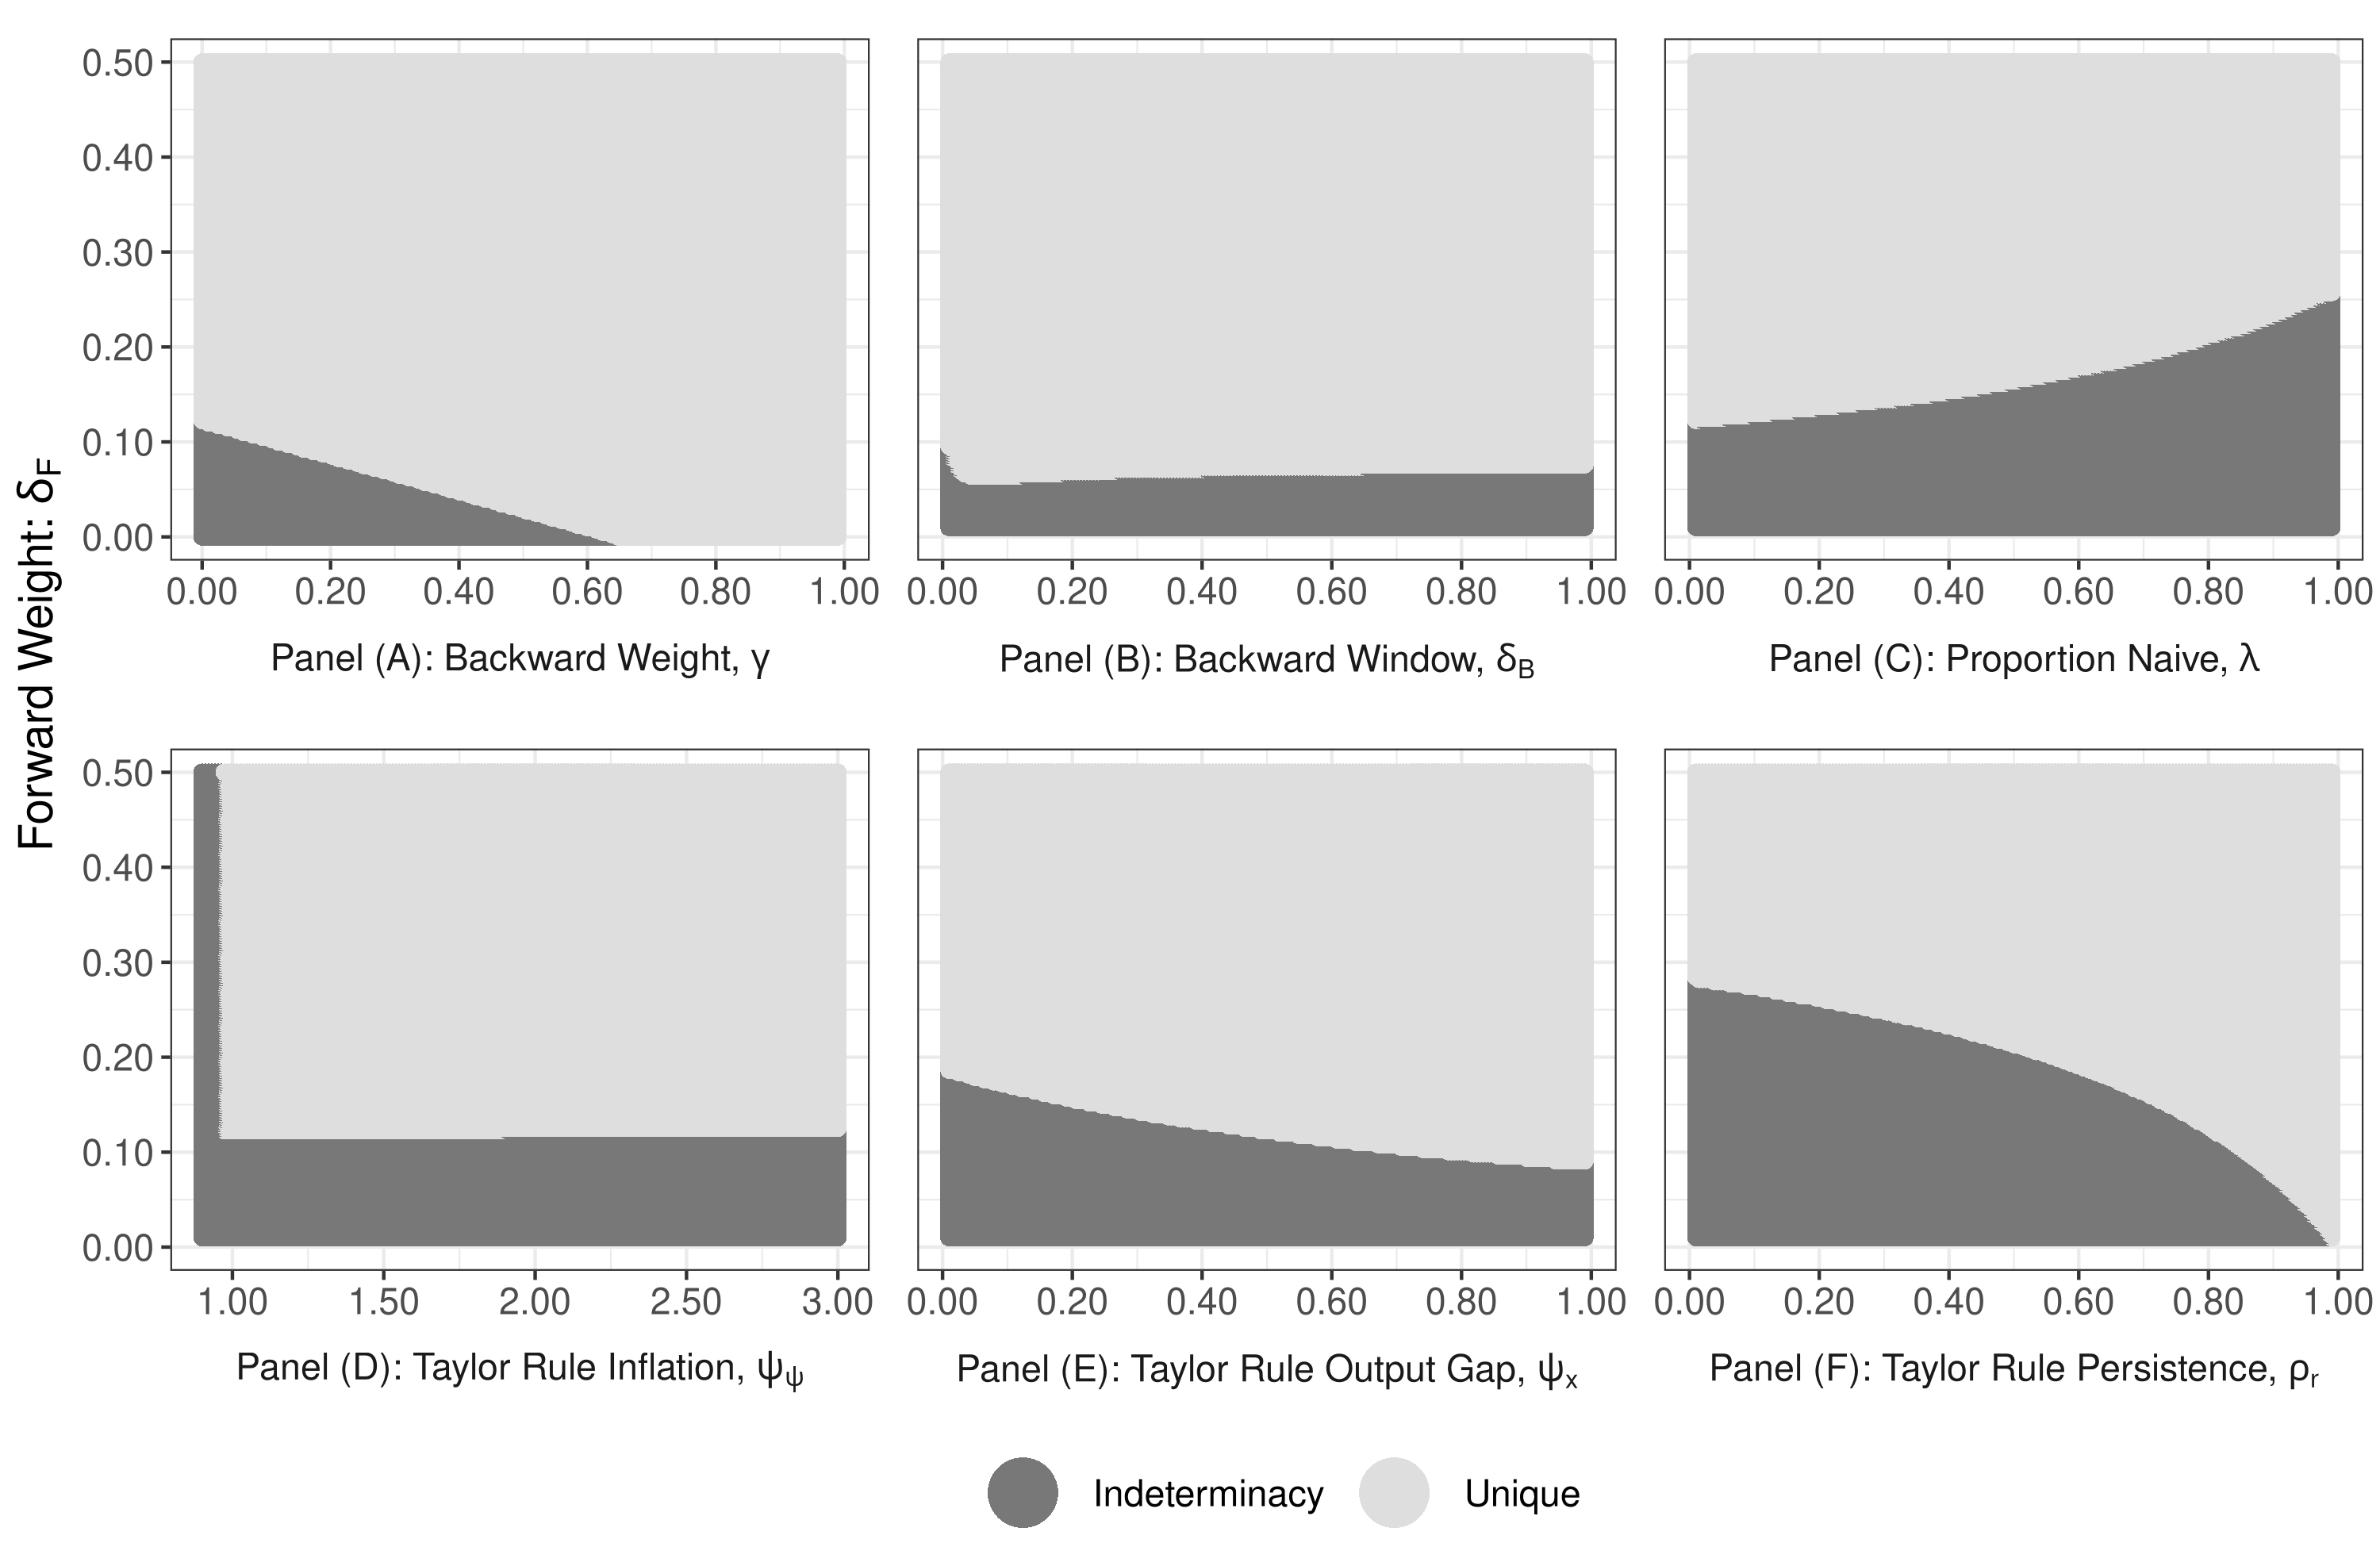
\includegraphics[width=\textwidth]{./determinacy_notitle.png}
		\vspace*{3pc}\hspace*{2pc}\parbox{0.9\textwidth}{\small{
			Notes: Larger values for $\delta_F$ imply shorter forward-looking windows. Other parameters not varying in each graph are given in \href{tb:parms}{Table} \ref{tb:parms}. In Panel (B), the baseline parameter for $\gamma$ is 0.25, implying a 25\% weight given to the backward-looking window versus the forward-looking window. In all other panels, the baseline parameter for $\gamma$ is equal to 0.0, implying purely forward-looking windows.}
		}
	\end{center}
	\vspace*{-4pc}\caption{Regions of Determinacy for Forward-Looking Windows}\label{fg:determinacy}
\end{figure}

\href{fg:determinacy}{Figure} \ref{fg:determinacy} shows the regions of determinacy for different values of the forward-looking weight, $\delta_F$, depending on four other parameters in the model. On the vertical axis in each panel are values for $\delta_F$ from 0.0 to 0.5. Given the inverse relationship between the weight on an individual observation and the length of a finite window, larger values for $\delta_F$ can be thought of as shorter forward-looking windows. The largest value considered, 0.5, approximates a forward-looking window of two quarters.

The first panel demonstrates the importance of using current or past values for inflation in the target window. When $\gamma=0.0$, no weight is put on past or current inflation, and the window is purely forward-looking. The smallest value for $\delta_F$ that delivers indeterminacy in this scenario is 0.12, so the largest possible forward-looking window is approximately 8.33 quarters, or just over two years. When $\gamma \geq 0.63$, all possible forward-looking windows yield determinate solutions. This implies, though, that the average inflation window has at least a 63\% weight on the current inflation rate, and therefore at most a 37\% weight on the forward window.

Panel (B) shows how the length of the backward-looking window affects determinacy. From Panel (A), we know that large weights placed on the backward-looking window can yield determinacy.\footnote{Not shown in the figure, we verified that when $\gamma=1.0$, implying that monetary policy has no forward-looking component, all values for $\delta_B\in[0,1]$ yield unique solutions.} We use a baseline value of $\gamma=0.25$ and find minimal variability in values of $\delta_F$ that yield determinacy. The most extreme value for $\delta_F$ yielding indeterminacy is 0.0933, implying that with 25\% weight put on the backward-window, the backward window can be as long as possible, and the forward-looking window can be as long as about $1/0.0933 = 10.7$ quarters.

Panel (C) shows that larger proportions of na\"ive agents lead to shorter lengths of forward-looking windows for determinacy. At the extreme, when nearly all agents are na\"ive, the smallest value $\delta_F$ can take is $0.255$, so the longest a forward-looking window can be in such a scenario is approximately $3.92$ quarters, just less than one year.

Panes (D), (E), and (F) show how the length of the forward-looking window depends on the Taylor Rule coefficients. Panel (D) shows that determinacy varies little with $\psi_\pi$. Panel (E) shows that as the Federal Reserve responds more strongly to the output gap, the longer it can make its forward-looking window (i.e. the smaller it can allow $\delta_F$). Panel (F) shows the important role persistence in monetary policy plays. The stronger is the level of persistence, the longer can be the forward looking window. At the extreme case when $\rho_r=0.0$, the smallest $\delta_F$ can be and still yield a determinant solution is $0.282$, implying forward-looking windows be no longer than approximately $3.55$ quarters.

\section{Conclusion}

The Federal Reserve's decision to engage in average inflation targeting has implications for monetary policy to avoid problems of indeterminacy, especially regarding the weight that the Fed puts on expected future values of inflation in its average inflation target. When little to no weight is put on past inflation, we find evidence that the Fed should restrict its forward looking window to less than two year to assure determinacy. When there is little persistence in the federal funds rate, we find evidence that the Fed should restrict its forward looking window to less than one year. We also find that when a large portion of economic agents form na\"ive expectations, the Fed should also restrict its forward-looking window to less than one year. When there is a high rate of persistence in monetary policy or the average inflation target is largely backward-looking, there are large ranges for average inflation targeting policy that lead to determinacy.

\bibliographystyle{apalike}
\bibliography{ait}

\end{document}
